\documentclass[letterpaper]{article}
\usepackage{aaai17}
\usepackage{times}
\usepackage{helvet}
\usepackage{courier}
\setlength{\pdfpagewidth}{8.5in}
\setlength{\pdfpageheight}{11in}

\usepackage[table]{xcolor}
\usepackage{listings}
\usepackage{amsmath}
\usepackage{tabularx}
\usepackage{graphicx}
\usepackage{hyperref}
\usepackage{cite}
\usepackage{float}
\usepackage{tikz}
\usetikzlibrary{shapes.geometric, arrows}
%\usepackage{authblk}
%\usepackage{fullpage}
%\usepackage{caption}
%\usepackage{subcaption}

\pdfinfo{
	/Title (Deep Learning Application in Collaborative Rating Prediction)
	/Author (Author 1, Author 2)
}
\lstset{language=python, tabsize=4}
\title{Deep Learning Application in Collaborative Rating Prediction}

\author{Author 1 \and Author 2\\
	Address line\\
	Address line\\
}

\begin{document}
\maketitle

\begin{abstract}
	Deep learning applications have become very successful in various domains 
	including image recognition, speech recognition and natural language 
	processing.
	However, the research on its application in recommendation systems is 
	still in early stage.
	Here we present Model R, a neural network model created to provide a deep 
	learning solution for collaborative rating prediction problem.
	This model extracts knowledge of users and items from known ratings and 
	uses this knowledge to predict unknown ratings.
	We demonstrate the power of Model R through experiments and compare it with 
	the most prevalent collaborative filtering algorithm - neighborhood-based 
	collaborative filtering.
	Model R proves deep learning can be successfully applied to collaborative 
	rating prediction problem and it outperforms neighborhood-based 
	collaborative filtering by up to 18\% in terms of prediction accuracy.
\end{abstract}

\section{Introduction}
The expression deep learning existed as early as 1986 in machine learning 
community \citeauthor{dechter1986learning}, though not so well known for many 
years.
But now, deep learning techniques using neural network models are rapidly 
gaining traction in more and more application domains 
such as:
\begin{itemize}
	\item speech recognition \citeauthor{hannun2014deep}
	\item image recognition \citeauthor{simonyan2014very}
	\item natural language processing \citeauthor{yao2013recurrent}
	\item graph mining \citeauthor{grovernode2vec}
	\item recommendation systems \citeauthor{barkan2016item2vec}
\end{itemize}
Two reasons for its adoptions in these domains are its higher prediction 
accuracy and less engineering compared to other machine learning techniques.
Among these domains, research in recommendation systems has been very active  
due to its extremely high value in industries such as search, e-commerce, 
travel and social \citeauthor{buettner2016predicting}.
Recommendation systems are classified into two groups according to the way they 
extract information about items: content based filtering and collaborative 
filtering \citeauthor{ricci2011introduction}.
Collaborative filtering extract information from the relations between users 
and items, while content based filtering extracts information from the contents 
of items.
Collaborative filtering has multiple forms including producing a list of items 
a user would like, and predicting the ratings a user would give to a list of 
items \citeauthor{su2009survey}.
The focus of this paper is the rating prediction form of collaborative 
filtering, which we call collaborative rating prediction.
The contribution of this paper is a deep learning application in 
collaborative rating prediction, which we believe is the first of its kind.

\section{Related work}
In this section,
we review a few existing deep learning applications in both content based 
filtering and collaborative filtering.
We also clarify how our work differs from these related work.

\subsection{Applications in content based filtering}
Applications in this group extract information of an item from its content, 
i.e., the input of the neural network is a vector produced from the item's 
content (e.g., the audio of a song, the text of an article). Here are some 
examples:
\begin{itemize}
	\item One example is a music recommendation system 
	\citeauthor{van2013deep}. 
	It is a tag prediction system implemented with a convolutional neural net: 
	the input is the spectrogram vector of the audio of a song, and the output 
	is the set of tags of the song (e.g., genre, instrumentation, tempo, mood).
	\item Another example is a multi-view recommendation system 
	\citeauthor{elkahky2015multi}. 
	It is a rating prediction system implemented with a fully connected neural 
	net: the input is the letter tri-gram vector of the text description of a 
	news article, app, etc, and the output is the rating.
\end{itemize}
Obviously, these applications are very similar to image recognition and speech 
recognition.
Our work differs from them in that our technique does not access the contents 
of items.

\subsection{Applications in collaborative filtering}
Applications in this group extract information of an item from its relations 
with other items, and the input of the neural net is a vector learned by the 
neural net itself from the relations between items.
All these applications treat a list of items as a sentence of words 
(effectively reducing their problems to a natural language processing problem)  
and then apply the skip-gram model used in word2vec 
\citeauthor{mikolov2013efficient}:
\begin{itemize}
	\item An item similarity prediction example is item2vec 
	\citeauthor{barkan2016item2vec} where purchase orders (lists of items) are 
	treated as sentences.
	\item Similar examples exist in graph mining, like deep walk 
	\citeauthor{perozzi2014deepwalk} and node2vec \citeauthor{grovernode2vec}, 
	where a 
	graph is sampled into walks (lists of nodes), and treated as sentences.
\end{itemize}
One drawback of these applications is that they fail to take advantage of 
the highly organized, regular and repeated structure in their relational data: 
relations between users and items (i.e., a user gives numerical rating to an 
item) and relations between nodes (i.e., a source node connects to a 
destination node though a labeled link).
This nice structure is not exploited in natural language processing because it 
does not exist (i.e., for a neural net, words can simply show up in a sequence 
from a day-to-day conversation, in many flexible and unpredictable ways, with 
little structure or regularity).
Although syntax and semantics exist in natural languages, we have not seen any 
current neural network models taking advantage of these structures.
Our work differs from the above applications in that our technique uses a 
neural net model designed to take advantage of the structure in the relational 
data and it is also able to predict a numerical attribute - the rating value.

\section{Problem}
The problem we consider in this paper is collaborative rating prediction 
problem.
In this section, we look at an example of the problem and then its definition.

\subsection{Problem example}
This is a collaborative rating prediction problem example: 
a set of 6 users give numerical ratings to a set of 3 items.
For each user, only a subset of his ratings are known; 
and we want to predict the unknown ratings.
The dataset of this example is demonstrated in \autoref{tab:ratings}.
\begin{table}[!htb]
	\centering
	\caption{The dataset of the problem example.
		In this dataset, a set of 6 users give ratings to a set of 3 items: 
		for User[0], ratings to all 3 items are known; 
		for User[1], ratings to Item[1] and Item[2] are known, 
		but the rating to Item[0] is unknown; and so on.
		Every unknown rating is marked as a question mark.
		The task is to predict the unknown ratings.
	}
	\begin{tabularx}{0.47\textwidth}{|X|c|c|c|}  \hline \rowcolor{blue!50}
		        & Item[0] & Item[1] & Item[2] \\ \hline
		User[0] & 3       & 5       & 2 \\ \hline
		User[1] & ?       & 5       & 2 \\ \hline
		User[2] & 4       & 4       & 5 \\ \hline
		User[3] & 2       & 4       & ? \\ \hline
		User[4] & 5       & 5       & 4 \\ \hline
		User[5] & 4       & ?       & 4 \\ \hline
	\end{tabularx}
	\label{tab:ratings}
\end{table}

\subsection{Problem definition}
Formally, a collaborative rating prediction problem is defined as follows:
\begin{itemize}
	\item given: a 2-D array R[m][n], 
	where R[i][j] is the rating User[i] gives to Item[j],
	$ i \in [0, m-1] $, j $ \in [0, n-1] $, and a number of elements in R are 
	unknown
	\item task: predict all unknown elements in R
\end{itemize}
Moreover, we define a user as the array of ratings he gives to all items:
\begin{align*}
	User[i] = R[i]
\end{align*}

\section{Baseline solutions}
Among many algorithms to collaborative rating prediction problem,
the most prevalent one is the neighborhood-based collaborative filtering 
algorithm \citeauthor{su2009survey}.
This algorithm also has several variants,
which we will use as baseline solutions.

\subsection{Algorithm}
The neighborhood-based collaborative filtering algorithm calculates each 
unknown R[i][j] as 
follows \citeauthor{su2009survey}:
\begin{align*}
R[i][j] = c \sum_{k = 0}^{m-1} S(i, k) R[k][j]
\end{align*}
where S(i, k) is the similarity of User[i] and User[k] to be defined by each 
variant,
unknown R[k][j]'s are omitted and c is a normalizing factor:
\begin{align*}
	c = \frac{1}{\sum_{l = 0}^{m - 1} |S(i, k)|}
\end{align*}
It is easy to understand the predicted rating R[i][j] as the sum of ratings all 
users give to Item[j],
weighted by how similar each user is to the target user.
The algorithm can opt to use only a fixed number of users with highest 
similarities to the target user in the calculation, instead of using all users.

\subsection{Variants}
Each variant of the algorithm has a unique definition of the similarity 
function of User[i] and User[k]:
\begin{itemize}
	\item PCC: The Pearson correlation coefficient similarity, defined as 
	\citeauthor{resnick1994grouplens}:
	\begin{align*}
		& S(x, y) \\
		=& S_{PCC}(x, y) \\
		=& \frac{\sum_{i \in I_{xy}}(R[x][i] - \overline{R[x]})(R[y][i] - 
		\overline{R[y]})}{\sum_{i \in I_{xy}}(R[x][i] - \overline{R[x]})^2 
		\sum_{i 
		\in I_{xy}}(R[y][i] - \overline{R[y]})^2 }
	\end{align*}
	where $ I_{x} $ is the set of items rated by User[x],
	and	$ \overline{R[x]} $ is the average rating User[x] gives to all items,
	and $ I_{xy} $ is the set of items rated by both User[x] and User[y].
	PCC measures the linear correlation of two users.
	\item WPCC: The weighted PCC similarity, defined as 
	\citeauthor{herlocker1999algorithmic}:
	\begin{align*}
		& S(x, y) \\
		=& S_{WPCC}(x, y) \\
		=&
		\begin{cases}
			\frac{|I_{xy}|}{T} S_{PCC}(x, y) & |I_{xy}| < T \\
			S_{PCC}(x, y) & otherwise
		\end{cases}
	\end{align*}
	where T is a threshold of number of items. 
	WPCC of two users differs from PCC only when the number of items rated by 
	both users (co-rated items) is less than the threshold. 
	When the difference occurs, less number of co-rated items results in less 
	similarity in the two users.
	\item SPCC: The sigmoid PCC similarity, defined as 
	\citeauthor{jamali2009trustwalker}:
	\begin{align*}
		& S(x, y) \\
		=& S_{SPCC} (x, y) \\
		=& \frac{S_{SPCC}(x, y)}{1 + exp(-\frac{|I_{xy}|}{2})}
	\end{align*}
	SPCC is very similar to WPCC in the sense two users have lower similarity 
	if they have a smaller number of co-rated items.
	\item MPCC: The multi-level PCC similarity \citeauthor{polatidis2016multi}. 
	This one is also very similar to the previous ones but much more complex, 
	so we skip its description here.
\end{itemize}

\section{Observations}
Although the various applications in related work section can not solve the 
collaborative rating prediction problem,
they all have an interesting key process: representing entities as vectors.
As deep learning techniques become more powerful and standardized, this key 
process seems to be the most significant part in a domain specific deep 
learning application.
In an informal way, that is like to say: in order to apply deep learning to a 
specific task, represent the data at hand as vectors of numbers,
feed them to the neural net, and then deep learning will take care of 
everything else.

\subsection{Entities and representations}
First of all, we summarize how a neural net represents various types of 
entities in different domains with different relations, as shown in 
\autoref{tab:domains}.
It is clear that representations for all the entities are numerical arrays, 
because neural nets rely on neurons' activations and communications, which 
are both numerical.
\begin{table}[!htb]
	\centering
	\caption{A summary of various types of entities, their numerical
		representations and inter-entity relations in different domains:
		Images in image recognition and audios in speech recognition can be 
		directly represented by 2D numerical arrays, 
		but their relations to other images or audios are not commonly 
		used. 
		Words in natural languages, items in recommendation systems, and nodes 
		in graphs can be represented by vectors (1D numerical arrays) and their 
		relations to other words, items and nodes are commonly used to learn 
		these vectors.}
	\begin{tabularx}{0.47\textwidth}{|X|c|c|} \hline \rowcolor{blue!50}
		Entity & Representation           & Relations \\ \hline
		image  & 2D light amplitude array & NA \\ \hline
		audio  & 2D sound amplitude array & NA \\ \hline
		word   & word vector              & co-occurrences \\ \hline
		item   & item vector              & co-purchases \\ \hline
		node   & node vector              & connections \\ \hline
	\end{tabularx}
	\label{tab:domains}
\end{table}

\subsection{Entities to vectors}
The word2vec technique is famous for using a neural net to learn to map every 
entity (word in this case) in a vocabulary to a vector without any domain 
knowledge \citeauthor{mikolov2013efficient}.
The subsequent techniques item2vec and node2vec use the same skip-gram 
model in word2vec to map items and nodes to vectors.
\autoref{tab:word} shows a mapping table that maps each entity(word/item/node) 
to its vector.
In a corpus, every word is described/defined only by related words in its 
contexts, by implicit relations between words in word co-occurrences.
Nonetheless, the neural net can learn from word co-occurrences and map words to 
vectors accordingly,
such that the relations between words are preserved in the word vector space 
\citeauthor{mikolov2013distributed}.
The same arguments apply to relations between items and nodes.
\begin{table}[!htb]
	\centering
	\caption{Entity (word/item/node) to vector mapping table for a set of n
		entities with entity vectors of size d:
		Each entity has an ID.
		The values of vectors in this table are hypothetical.
		}
	\begin{tabularx}{0.47\textwidth}{|c|X|} \hline \rowcolor{blue!50}
		Entity ID & Entity (word/item/node) vector \\ \hline
		1         & [2.3, 564, -9.5 ... 3] \\ \hline
		2         & [76, -342.2, 0.3 ... 4.2] \\ \hline
		3         & [-345, -834, 0.3 ... 34] \\ \hline
		...       & ... \\ \hline
		n         & $ [x_1, x_2, x_3 ... x_d] $ \\ \hline
	\end{tabularx}
	\label{tab:word}
\end{table}

\subsection{Users and items to vectors}
However, the relation between a user and an item is quite different from that 
between words:
\begin{itemize}
	\item The rating a user gives to an item explicitly tells us how much the 
	user likes that item;
	the relation is very specific: one user, one item, one rating - no more, no 
	less.
	\item The co-occurrences of words [the, quick, brown, fox, jumps, over] 
	implicitly tell us these words are related but do not tell us any specific 
	relation.
\end{itemize}
This observation suggests that a neural net should be able to learn user to 
vector mapping and item to vector mapping supervised by the rating, in a more 
specific, direct and simply way than it learns word to vector mappings 
supervised by word co-occurrences.

\section{Solution}
Following the above observations, we can build an estimator with a neural net 
model using a (user, item) pair as its input and the rating as its output.
Therefore, we should change the format of the example dataset from the one 
shown in \autoref{tab:ratings} to a new one shown in \autoref{tab:rating}.
The estimator will train on entries with known ratings (the train set) 
and predict on the entries with unknown ratings (the test set).
Of course our testing program knows the unknown ratings in order to calculate 
the model's prediction error.
\begin{table}[!htb]
	\centering
	\caption{The reformatted dataset of the problem example.}
	\begin{tabularx}{0.47\textwidth}{|c|X|}  \hline \rowcolor{blue!50}
		Input = (User ID, Item ID) & Output = Rating \\ \hline
		(0, 0)                     & 3 \\ \hline
		(0, 1)                     & 5 \\ \hline
		(0, 2)                     & 2 \\ \hline
		(1, 0)                     & ? \\ \hline
		...                        & ... \\ \hline
	\end{tabularx}
	\label{tab:rating}
\end{table}

\subsection{Conceptual neural net model}
The model in the estimator is a fully connected neural net which we call Model 
R (R as in relation), shown in \autoref{fig:conceptural}.
\begin{figure*}[!htb]
	\centering
	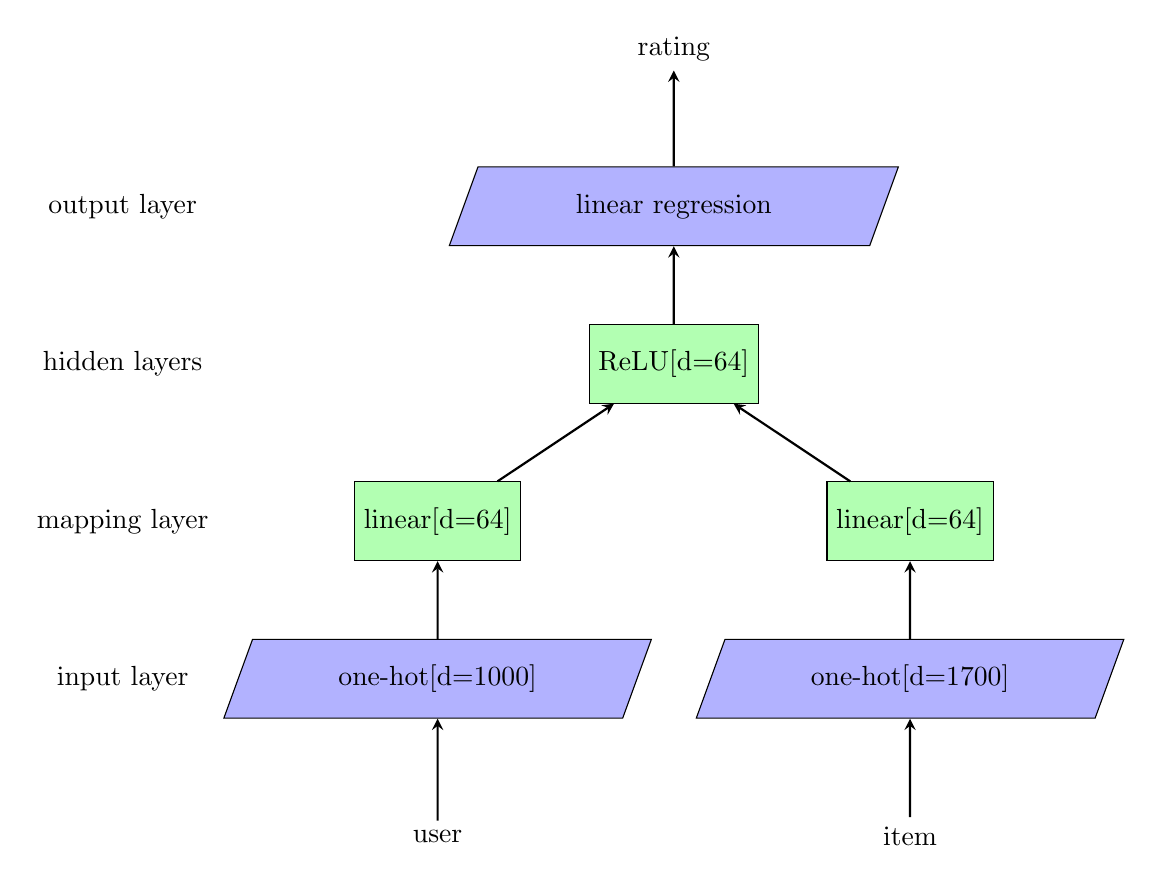
\begin{tikzpicture}[node distance=2cm]
	\tikzstyle{io} = [trapezium, trapezium left angle=70, trapezium right 
	angle=110, minimum width=1cm, minimum height=1cm, text centered, 
	draw=black, fill=blue!30]
	\tikzstyle{process} = [rectangle, minimum width=1cm, minimum height=1cm, 
	text centered, draw=black, fill=green!30]
	\tikzstyle{arrow} = [thick,->,>=stealth]
	\node (linearRegression) [io] {linear regression};
	\node (relu3) [process, below of=linearRegression] {ReLU[d=64]};
	\node (linear1) [process, below of=relu3, xshift=-3cm] {linear[d=64]};
	\node (linear2) [process, below of=relu3, xshift=3cm] {linear[d=64]};
	\node (oneHot2) [io, below of=linear2] {one-hot[d=1700]};
	\node (oneHot1) [io, below of=linear1] {one-hot[d=1000]};
	\node (rating) [above of=linearRegression] {rating};
	\node (output) [left of=linearRegression, xshift=-5cm] {output layer};
	\node (hidden1) [below of=output] {hidden layers};
	\node (mapping) [below of=hidden1] {mapping layer};
	\node (input) [below of=mapping] {input layer};
	\node (user) [below of=oneHot1] {user};
	\node (item) [below of=oneHot2] {item};
	\draw [arrow] (user) -- (oneHot1);
	\draw [arrow] (item) -- (oneHot2);
	\draw [arrow] (oneHot1) -- (linear1);
	\draw [arrow] (oneHot2) -- (linear2);
	\draw [arrow] (linear1) -- (relu3);
	\draw [arrow] (linear2) -- (relu3);
	\draw [arrow] (relu3) -- (linearRegression);
	\draw [arrow] (linearRegression) -- (rating);
	\end{tikzpicture}
	\caption{The conceptual model R for a dataset with 1700 items and 1000 
	users:
	The d in the bracket (d as in dimension) is the layer's size (number of 
	units in the layer).
	We keep all layers the same size for simplicity, although layers of 
	different sizes may produce better results.
	The text before the bracket refers to the activation function of the 
	units in the layer (except for one-hot, which refers to the activations 
	in the input layer).
	Only layers and their connections are shown, while the units in each 
	layer and their connections are not shown.
	}
	\label{fig:conceptural}
\end{figure*}
The model contains the following layers:
\begin{itemize}
	\item an input layer with one-hot activations: it has 1 channel for items 
	and 1 channel for users;
	this layer is directly activated by the testing program (e.g., to feed the 
	1200th item, the testing program sets 1 at the 1200th unit and 0 at other 	
	units in the item channel);
	\item a mapping layer with linear units: it has one channel to map each 
	entity to a vector;
	the activations of these two channels are the two vectors;
	it is the most critical layer as it gradually learns to map users and items 
	to vectors, which are complex and unobservable user and item attributes
	\item several fully connected hidden layers (1 layer is shown in the figure;
	multiple numbers of layers and layer sizes are considered in the 
	experiments) of ReLU (rectified linear units):
	they have non-linear activation functions to give the model sufficient 
	complexity;
	they learn to extract more and more abstract rating-relevant information;
	\item an output layer with a linear regression unit: it learns to predict 
	the rating based on abstracted information;
\end{itemize}
In this problem, ratings provide the all information about users and items.
We fully take this character into account and design this model to learn 
complex and unobservable user and item attributes (i.e., user and item vectors) 
supervised by simple and observable rating.

\subsection{Actual neural net model}
In practice, Model R uses more efficient mapping tables instead of a 
one-hot input layer to handle a dataset with increasing number of users and 
items.
\autoref{fig:actural} shows the actual model with two modifications from the 
conceptual model:
\begin{itemize}
	\item The input layer is replaced by two mapping tables: one for users and 
	one for items;
	their inputs are user and item IDs and their outputs are user and item 
	vectors, just like the entity to vector mapping table referenced in 
	\autoref{tab:word}
	\item The mapping layer is replaced by a 2-channel input layer: it is 
	directly activated by the outputs of the mapping tables
\end{itemize}
\begin{figure*}[!htb]
	\centering
	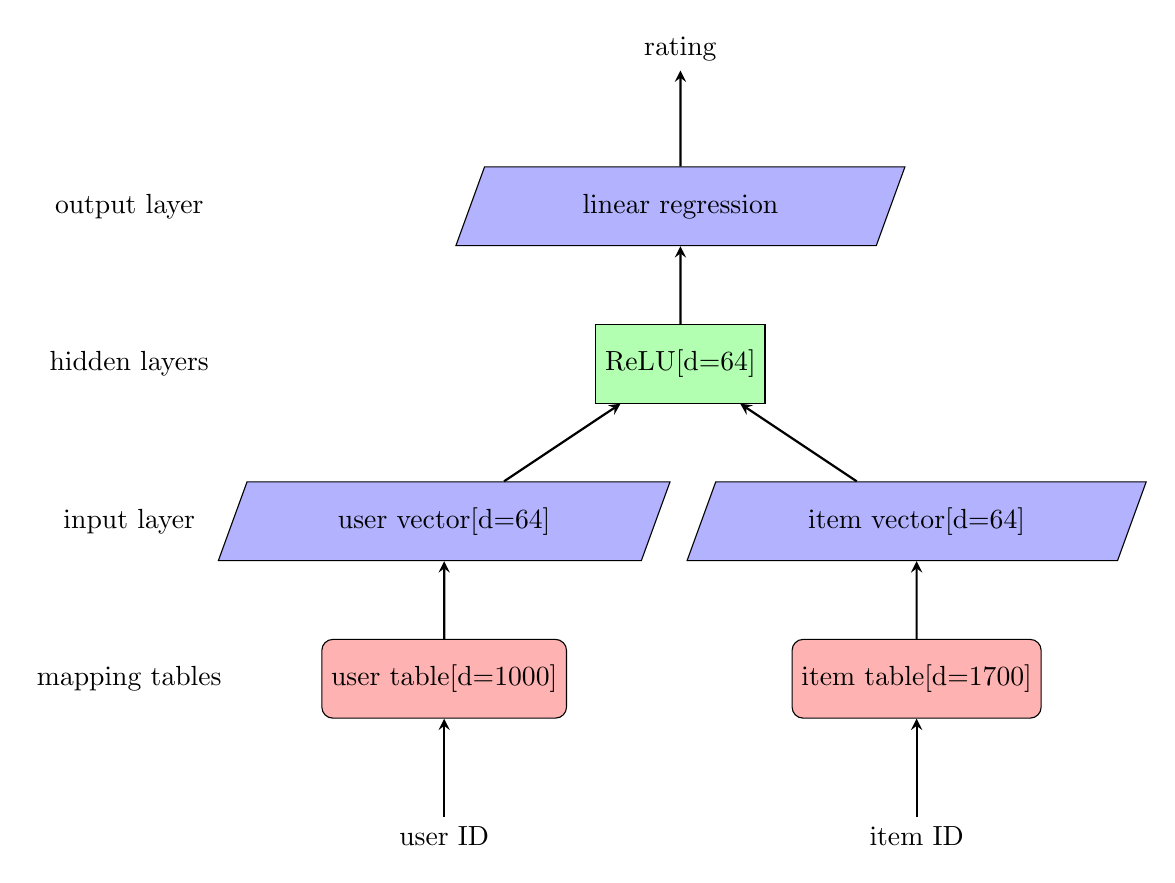
\begin{tikzpicture}[node distance=2cm]
	\tikzstyle{io} = [trapezium, trapezium left angle=70, trapezium right 
	angle=110, minimum width=1cm, minimum height=1cm, text centered, 
	draw=black, fill=blue!30]
	\tikzstyle{startstop} = [rectangle, rounded corners, minimum width=1cm, 
	minimum height=1cm, text centered, draw=black, fill=red!30]
	\tikzstyle{process} = [rectangle, minimum width=1cm, minimum height=1cm, 
	text centered, draw=black, fill=green!30]
	\tikzstyle{arrow} = [thick,->,>=stealth]
	\node (linearRegression) [io] {linear regression};
	\node (relu3) [process, below of=linearRegression] {ReLU[d=64]};
	\node (linear1) [io, below of=relu3, xshift=-3cm] {user vector[d=64]};
	\node (linear2) [io, below of=relu3, xshift=3cm] {item vector[d=64]};
	\node (oneHot1) [startstop, below of=linear1] {user table[d=1000]};
	\node (oneHot2) [startstop, below of=linear2] {item table[d=1700]};
	\node (rating) [above of=linearRegression] {rating};
	\node (output) [left of=linearRegression, xshift=-5cm] {output layer};
	\node (hidden1) [below of=output] {hidden layers};
	\node (input) [below of=hidden1] {input layer};
	\node (mapping) [below of=input] {mapping tables};
	\node (user) [below of=oneHot1] {user ID};
	\node (item) [below of=oneHot2] {item ID};
	\draw [arrow] (user) -- (oneHot1);
	\draw [arrow] (item) -- (oneHot2);
	\draw [arrow] (oneHot1) -- (linear1);
	\draw [arrow] (oneHot2) -- (linear2);
	\draw [arrow] (linear1) -- (relu3);
	\draw [arrow] (linear2) -- (relu3);
	\draw [arrow] (relu3) -- (linearRegression);
	\draw [arrow] (linearRegression) -- (rating);
	\end{tikzpicture}
	\caption{The actual model with two modifications:
		We factor the entity vector mapping process out of the neural net into 
		2 mapping tables.
		We feed every item or user to the estimator by feeding the ID.
		During learning, the estimator updates the vectors in the tables the 
		same way it updates weights in the conceptual model.}
	\label{fig:actural}
\end{figure*}

\subsection{Learning algorithms and techniques}
The estimator uses the above model and a number of popular deep learning 
algorithms and techniques:
\begin{itemize}
	\item backpropagation: propagation of the error gradients from output layer 
	back to each earlier layer \citeauthor{rumelhart1988learning}
	\item stochastic gradient descent: the optimization that minimizes 
	the error (descending against the error gradient in weight space) for a 
	random sample in each step \citeauthor{lecun2012efficient}
	\item mini-batch: the modification to stochastic gradient descent to 
	accelerate and smooth the descent by minimizing the error for a small 
	random batch of samples in each step \citeauthor{mairal2010online}
\end{itemize}

\section{Experiments}
We evaluated Model R and the baseline solutions experimentally,
and the results showed that Model R achieved much lower prediction error than 
the baseline solutions.

\subsection{Experiment settings}
We evaluated Model R in the same settings used in a recent experimental 
evaluation of the baseline solutions \citeauthor{polatidis2016multi},
one experiment for each of the four datasets 
(Jester \citeauthor{goldberg2001eigentaste} is not used due to its non-standard 
file 
formatting issue): 
\begin{itemize}
	\item ML100K: MovieLens100K\citeauthor{harper2015movielens}
	\item ML1M: MovieLens1M\citeauthor{harper2015movielens}
	\item EP: Epinions \citeauthor{massa2007trust}
	\item MT: MovieTweetings \citeauthor{dooms2013movietweetings}
\end{itemize}
The specifications of the datasets are summarized in \autoref{tab:dataset}.
The experiments use MAE (mean absolute error) as the prediction accuracy 
metric, and split each dataset into 2 parts: 20\% into the test set and 80\% 
into the training set.
\begin{table}[!htb]
	\centering
	\caption{The dataset specs: 
		The three columns are the dataset, number of users, items and ratings 
		of the dataset.
		}
	\begin{tabularx}{0.47\textwidth}{|X|X|X|X|}  \hline \rowcolor{blue!50}
		Dataset & User \# & Item \# & Rating \# \\ \hline
		ML100K  & 1,000   & 1,700   & 100,000 \\ \hline
		ML1M    & 6,000   & 4,000   & 1,000,000 \\ \hline
		EP      & 49,290  & 139,738 & 664,824 \\ \hline
		MT      & 39,363  & 22,610  & 431,780 \\ 
		\hline
	\end{tabularx}
	\label{tab:dataset}
\end{table}

\subsection{Experiment process}
At the beginning of an experiment on a dataset,
the estimator sets aside 10\% of the training set as a validation set.
A larger or smaller validation set could not reduce the prediction error in the 
experiments.
Then the estimator learns for several epochs:
in each epoch, it learns on training set, predicts on validation set, and logs 
the validation error.
In order to reduce over-fitting, the estimator stops learning when the 
validation error has not decreased for 3 epochs.
At the end, the testing program lets the estimator predict on testing set and 
record its testing error as its prediction error on that dataset.

\subsection{Experiment results}
In our experiments, Model R's prediction error is 18\% to 8\% lower than
the best baseline solution MPCC - on all datasets, shown in 
\autoref{tab:errors}.
The error reduction from MPCC to Model R is calculated as:
\begin{align*}
	\delta = 1 - \frac{MPCCError}{ModelRError}
\end{align*}
\begin{table}[!htb]
	\centering
	\caption{The comparison of prediction errors (measured by MAE): 4 baseline
		solutions are represented by their first letters (P, W, S, M).
		Model R (represented by letter R)'s prediction error is 18\% to 8\% 
		lower than the best baseline 
		solution (MPCC) on all datasets.
		}
	\begin{tabularx}{0.47\textwidth}{|X|c|c|c|c|c|c|} \hline 
	\rowcolor{blue!50}
		Dataset & P    & W    & S    & M    & R    & $ \delta $ \\ \hline
		ML100K  & 0.83 & 0.82 & 0.83 & 0.82 & 0.70 & 14\% \\ \hline
		ML1M    & 0.83 & 0.81 & 0.83 & 0.79 & 0.65 & 17\% \\ \hline
		EP      & 1.00 & 1.02 & 1.00 & 0.93 & 0.76 & 18\% \\ \hline
		MT      & 1.38 & 1.32 & 1.33 & 1.26 & 1.15 & 8\%  \\ \hline
	\end{tabularx}
	\label{tab:errors}
\end{table}
Model R is also very robust - 4\% fluctuation in prediction error - in a wide 
parameter ranges listed below:
\begin{itemize}
	\item number of hidden layers: [2, 5]
	\item layer size: [20, 90]
	\item learning rate: [0.01, 0.1]
	\item batch size: [30, 70]
\end{itemize}

\subsection{Computing resources}
We ran our experiments on a Dell Optiplex 780 machine with following 
configurations:
\begin{itemize}
	\item operating system: Ubuntu 16.04 64-bit
	\item processor: Intel Core 2 Duo CPU E8400 @ 3GHz
	\item memory: 4GB
\end{itemize}
Each run (learning and prediction) takes around 1 to 8 minutes, 4 to 16 epochs, 
depending on the dataset and parameters.
Our implementation exploits thread level parallelism, but we have not explored 
data level parallelism (i.e., GPU) or process level parallelism (e.g., remote 
procedure call).

\section{Future work}
We designed Model R for collaborative rating prediction problem,
but we would like to incorporate content based capability into it to improve 
its prediction accuracy.
For example, in order to better predict the rating a user gives to an article,
the model can append units at the mapping layer to receive a content vector 
mapped from the text of the article by another neural net.
The model can also append one unit for each numerical attribute of the user or 
item (e.g., the age of a user, the price of a product) at the mapping layer.
In this way, it will take advantage of not only relation data but also content 
data, and therefore make more accurate predictions.
We have an open source Python implementation under MIT license hosted on Github 
(url omitted to comply with AAAI review requirements).
The main machine learning package we use is TensorFlow 
\citeauthor{abadi2016tensorflow}.
Do not hesitate to contact us if you are interested in collaboration.

\section{Conclusions}
Model R proves deep learning can be successfully applied to collaborative 
rating prediction problem and it can provide a solution to achieve higher 
prediction accuracy than the most prevalent collaborative filtering algorithm.
The estimator powered by Model R effectively learns complex and unobservable 
user and item attributes from simple and observable relations (i.e., users rate 
items).
The estimator learns both to map each entity to a vector, and to predict 
the rating using these vectors.

\bibliographystyle{aaai}
\bibliography{references}
\end{document}
